\section{Background}\label{sec:Background}

This section describes the memory management model and guard mechanism in CRuby. We first explain how Ruby objects own native memory regions and how subordinate pointers are obtained from them. We then describe the compiler optimizations that can shorten the lifetime of owning references, and CRuby's conservative scanning strategy. Finally, we present the \texttt{RB\_GC\_GUARD} mechanism and discuss why correct placement is both critical and difficult.

\subsection{Subordinate Memory in CRuby}
Non-immediate CRuby objects occupy a fixed-size slot (header) in the GC heap. If the payload fits within this slot, it is stored internally; otherwise, the header points to an additional region of native memory.  The GC tracks the header as a Ruby object, but the payload typically resides in memory areas managed by CRuby's runtime and reclaimed when the owning object is reclaimed.  We call such payload regions \emph{subordinate memory areas}.

A \emph{subordinate pointer} is a raw C pointer that points into subordinate memory.  It is \emph{not} a Ruby object and therefore is not treated as a GC root.  Subordinate pointers are pervasive in the interpreter and in C extensions because they are the conventional way to access Ruby payloads. However, because they are ordinary C pointers, their validity depends on the liveness of the owning Ruby object.

For example, in the case of strings, the standard subordinate pointer derivation operation is \texttt{RSTRING\_PTR(str)},
which returns a \texttt{char *} pointing to the string's bytes.  

\subsubsection*{Subordinate Accessing Example}
Subordinate pointers are the standard way C code accesses Ruby object data.  Listing~\ref{lst:derived_ptr_pattern} shows a typical pattern: obtain a Ruby string and derive a pointer to its bytes via \texttt{RSTRING\_PTR}.  This pattern pervades both the CRuby interpreter and C extensions.

\begin{figure}[tb]
\begin{lstlisting}[caption={Typical subordinate pointer access pattern.},label={lst:derived_ptr_pattern}]
VALUE path = rb_iseq_path(iseq);
const char *ptr = RSTRING_PTR(path);
long len = RSTRING_LEN(path);
/* ptr now points to path's bytes; use in C operations */
memcmp(ptr, "-e", 2);
\end{lstlisting}
\end{figure}

Because subordinate pointers are not GC roots, and because compilers may treat the owning
\texttt{VALUE} as dead once the last \texttt{VALUE}-level use has occurred, code that
uses subordinate pointers across allocation-heavy calls is particularly susceptible to the
Guard Problem discussed in Section~\ref{sec:guard_problem}.

\subsection{Conservative Stack Scanning of CRuby's GC}
CRuby uses conservative scanning for GC roots. Under this strategy, whether a Ruby object is retained depends on whether some machine-state location still contains a bit pattern that looks like a pointer to the object. If an optimizing compiler shortens the lifetime of the owning \texttt{VALUE} variable and reuses its storage, the pointer to the object may get overwritten and become invisible to the collector even though subordinate pointers into its subordinate memory are still in use. Such compiler optimizations will be discussed in Section \ref{sec:compiler_opts}.


\subsection{The \texttt{RB\_GC\_GUARD} Mechanism}
To prevent subordinate pointers from outliving their owning \texttt{VALUE} under these optimizations, CRuby exposes the macro \texttt{RB\_GC\_GUARD} as an explicit optimization barrier. With GCC, \texttt{RB\_GC\_GUARD} is implemented by creating a \texttt{volatile VALUE *} pointing to \texttt{v} and issuing an empty inline assembly statement with a memory constraint, making the access appear as an observable side effect that must not be optimized away. CRuby's documentation recommends \texttt{RB\_GC\_GUARD} over using \texttt{volatile} directly, because the macro localizes the optimization impact to the guard site~\cite{ruby_capi_rb_gc_guard}. The implementation of \texttt{RB\_GC\_GUARD} for GCC is shown in Listing~\ref{lst:rbgcguard}. Since the CodeQL database used in our analysis is built with GCC, our analysis considers only this implementation.

\begin{figure}[tb]
\begin{lstlisting}[caption={RB\_GC\_GUARD's Definition (GCC)},label={lst:rbgcguard}]
#define RB_GC_GUARD(v) \
    (*__extension__ ({ \
        volatile VALUE *rb_gc_guarded_ptr = &(v); \
        __asm__("" : : "m"(rb_gc_guarded_ptr)); \
        rb_gc_guarded_ptr; \
    }))
\end{lstlisting}
\end{figure}

\subsection{Compiler Optimizations}\label{sec:compiler_opts}
Optimizing compilers may keep a local variable only as long as it is needed for C-level computations. When the last use of a \texttt{VALUE} has passed, the compiler may reuse the same register or stack location for other values. This can break GC safety when code derives a subordinate pointer from a Ruby object and later uses that pointer after the owning \texttt{VALUE} is no longer kept in the machine state.

Compiler optimizations based on variable liveness often lead to the Guard Problem. After extracting a derived pointer \texttt{p} from a \texttt{VALUE v} (e.g., \texttt{p = RSTRING\_PTR(v)}), the compiler may treat \texttt{v} as "dead" if it is not referenced again. As a result, the register or stack slot holding \texttt{v} is reused for other data. This occurs in optimizations such as GCC's \texttt{-fstack-reuse}\cite{gcc_fstack_reuse} and LLVM's Stack Coloring\cite{llvm_stack_coloring}. In a conservative GC setup, this reuse may overwrite the original \texttt{VALUE}, making the object unreachable even while the derived pointer \texttt{p} is still in use.

\texttt{RB\_GC\_GUARD} addresses this by forcing a use of the \texttt{VALUE} at an explicit program point. When placed after calls that may trigger GC, the forced use makes the compiler keep the \texttt{VALUE} until that point, typically by storing it in a stack slot that remains visible to conservative scanning.

We confirmed this behavior in a compiled CRuby routine. We built CRuby 3.4.5 (\texttt{-O3}, x86\_64) with GCC 15.2.1 and inspected \texttt{rb\_marshal\_dump\_limited} in \texttt{marshal.c} (Appendix~\ref{app:rb_marshal_dump_limited}). The function allocates a typed-data wrapper Ruby object \texttt{wrapper} and derives \texttt{arg}, a raw pointer into that object's payload. Because \texttt{arg} is a plain C pointer, it does not keep \texttt{wrapper} reachable under conservative scanning; \texttt{wrapper} must remain visible in a register or stack slot across later calls.

Listing~\ref{lst:asm_rb_marshal_dump_limited} shows the disassembly around the allocation and the return sequence. In the original build (top), the \texttt{wrapper} value returned in \texttt{rax} is stored to \texttt{[rsp+0x8]} immediately after \texttt{rb\_data\_typed\_object\_zalloc}. The next call overwrites \texttt{rax}, but the stack slot still holds \texttt{wrapper}. Near the return, \texttt{RB\_GC\_GUARD(wrapper)} forces an access to the same stack slot. In the variant where only \texttt{RB\_GC\_GUARD(wrapper)} is removed (bottom), GCC does not store \texttt{wrapper} to the stack: the next call overwrites \texttt{rax}, and \texttt{[rsp+0x8]} is used only for the stack-protection value. As a result, there is no remaining copy of \texttt{wrapper} in the scanned machine state while \texttt{arg} is still used.

\begin{figure}[tb]
\begin{lstlisting}[caption={Disassembly excerpts of \texttt{rb\_marshal\_dump\_limited} (GCC 15.2.1, x86\_64, \texttt{-O3}). Top: original with \texttt{RB\_GC\_GUARD(wrapper)}; bottom: guard removed and rebuilt.},label={lst:asm_rb_marshal_dump_limited}]
00000000001c7410 <rb_marshal_dump_limited>:
  1c7427:	sub    rsp,0x28
  1c742b:	mov    r14,QWORD PTR fs:0x28
  1c7434:	mov    QWORD PTR [rsp+0x18],r14
  1c743c:	lea    rdx,[rip+0x4d70dd]        # 69e520 <dump_arg_data>
  1c7443:	call   16c350 <rb_data_typed_object_zalloc>
  1c7448:	lea    rbx,[rax+0x20]
  1c744c:	test   BYTE PTR [rax+0x18],0x2
  1c7450:	jne    1c7456 <rb_marshal_dump_limited+0x46>
  1c7452:	mov    rbx,QWORD PTR [rax+0x20]
  1c7456:	mov    QWORD PTR [rbx+0x8],0x0
  1c745e:	mov    QWORD PTR [rsp+0x8],rax
  1c7463:	call   2beb90 <rb_st_init_numtable>
  1c7468:	mov    QWORD PTR [rbx+0x10],rax
  1c746c:	call   184b70 <rb_init_identtable>

  1c75cc:	lea    rax,[rsp+0x8]
  1c75d1:	mov    QWORD PTR [rsp+0x10],rax
  1c75d6:	mov    rax,QWORD PTR [rsp+0x8]
  1c75db:	mov    rax,QWORD PTR [rsp+0x18]
  1c75e0:	sub    rax,QWORD PTR fs:0x28

00000000001c7410 <rb_marshal_dump_limited>:
  1c7427:	sub    rsp,0x18
  1c742b:	mov    r14,QWORD PTR fs:0x28
  1c7434:	mov    QWORD PTR [rsp+0x8],r14
  1c743c:	lea    rdx,[rip+0x4d70dd]        # 69e520 <dump_arg_data>
  1c7443:	call   16c350 <rb_data_typed_object_zalloc>
  1c7448:	lea    rbx,[rax+0x20]
  1c744c:	test   BYTE PTR [rax+0x18],0x2
  1c7450:	jne    1c7456 <rb_marshal_dump_limited+0x46>
  1c7452:	mov    rbx,QWORD PTR [rax+0x20]
  1c7456:	mov    QWORD PTR [rbx+0x8],0x0
  1c745e:	call   2beb90 <rb_st_init_numtable>
  1c7463:	mov    QWORD PTR [rbx+0x10],rax
  1c7467:	call   184b70 <rb_init_identtable>

  1c75c7:	mov    rax,QWORD PTR [rsp+0x8]
  1c75cc:	sub    rax,QWORD PTR fs:0x28
\end{lstlisting}
\end{figure}


\subsection{The Guard Problem}\label{sec:guard_problem}

\begin{figure}[tb]
\begin{lstlisting}[caption={The Guard Problem},label={lst:guard_problem}]
VALUE str = rb_str_new_cstr("Hello");
char *ptr = RSTRING_PTR(str);
rb_ary_push(array, other_value);
// may trigger GC
printf("%s\n", ptr);
// use after potential GC
\end{lstlisting}
\end{figure}

Manual \texttt{RB\_GC\_GUARD} placement is error-prone because developers must identify subordinate pointer derivations, potential GC triggers, and the temporal coverage needed for the subordinate pointer's lifetime.  GC may not run even when a trigger site is reached, making bugs hard to reproduce. We refer to this as the Guard Problem.

Moreover, bugs caused by omitted guards are difficult to debug because GC timing is non-deterministic. An omitted guard creates a \emph{possibility} of use-after-free, but a crash only occurs if a GC cycle is triggered at the buggy point \emph{and} the compiler has optimized away the root reference. As a result, code may pass testing for years and fail only under certain build configurations or high memory pressure, making these bugs hard to reproduce and diagnose.

Traditional static analyses for use-after-free in C/C++~\cite{static_analysis_use_after_free_cpp,spatio_temporal_context_reduction,static_analysis_dangling_pointer} do not directly address this conservative-GC setting.

\subsection{Performance Impact of Guards}\label{sec:Benchmark}

\texttt{RB\_GC\_GUARD} itself looks ``free'' because the implementation for use with GCC expands to an empty inline assembly statement.  However, its purpose is to \emph{change} the compiler's optimization decisions: it forces an observable use of the guarded \texttt{VALUE} at the guard site. Concretely, the macro takes the address of the \texttt{VALUE}, stores it through a \texttt{volatile VALUE *}, and feeds that pointer to an inline-assembly operand with a memory constraint~\cite{ruby_capi_rb_gc_guard} (see Listing~\ref{lst:rbgcguard}). This makes the guarded variable \emph{address-taken} and therefore typically forces it to be materialized in a stack slot (so that \texttt{\&(v)} is meaningful), and it can induce an extra post-trigger reload from that slot. In optimized builds, these constraints increase register pressure and can introduce spill/reload traffic, inhibit stack-slot reuse and tail-call optimization, and block otherwise-valid code motion.

Guarding can also affect performance indirectly through CRuby's conservative root discovery.  Conservative stack scanning is linear in the amount of native stack memory that is considered ``in use.''  When guards force more locals to be kept in stack slots (and, in the ``guard-everything'' configuration, extend live ranges to the end of a scope), they can increase both the number of machine words that must be scanned at each GC and the number of accidental pointer-shaped values that retain objects, delaying reclamation.  Thus, even though \texttt{RB\_GC\_GUARD} is not a GC call, indiscriminate use can increase GC work and memory retention.

To solve the problem of omitted guards, a naive strategy is to add \texttt{RB\_GC\_GUARD} to every \texttt{VALUE} variable. To assess practicality, we instrumented CRuby to apply \texttt{RB\_GC\_GUARD} broadly and ran \texttt{ruby-bench} as of commit e1e2ae3 \footnote{\url{https://github.com/ruby/ruby-bench/tree/e1e2ae32a3f8f003adf3c1a8ec4baca77dc4c091}}, the benchmark suite used by CRuby developers, comparing the instrumented build against the unmodified baseline. All benchmark measurements were obtained on a desktop equipped with an AMD Ryzen 7 5700X3D CPU.

To make this ``guard-everything'' configuration reproducible without manual editing, we generated the instrumentation mechanically. We first ran a CodeQL query to enumerate local variables whose declared type is \texttt{VALUE} and to locate the end of each variable's lexical scope in the C AST (i.e., the closing brace of the smallest enclosing compound statement that defines the variable's lifetime). The query emits the source file and line/column coordinates of each scope end together with the variable name. A small Python source-to-source rewriting script then applies these edits by inserting \texttt{RB\_GC\_GUARD(v);} immediately before the corresponding scope end (skipping sites that already contain an explicit guard for the same variable). Both the original CRuby and the guard inserted CRuby are compiled using the same compiler options (GCC, -O3 enabled). This produces a consistent instrumented variant that approximates an upper bound on the optimization impact of pervasive guarding.

We observed benchmark-dependent effects. In our setup, the geometric mean performance difference was approximately 6.99\% across the suite (positive indicates slowdown), with a maximum slowdown of 32.54\%. Figure~\ref{fig:benchmark_comparison} summarizes the results.

\begin{figure}[ht]
\centering
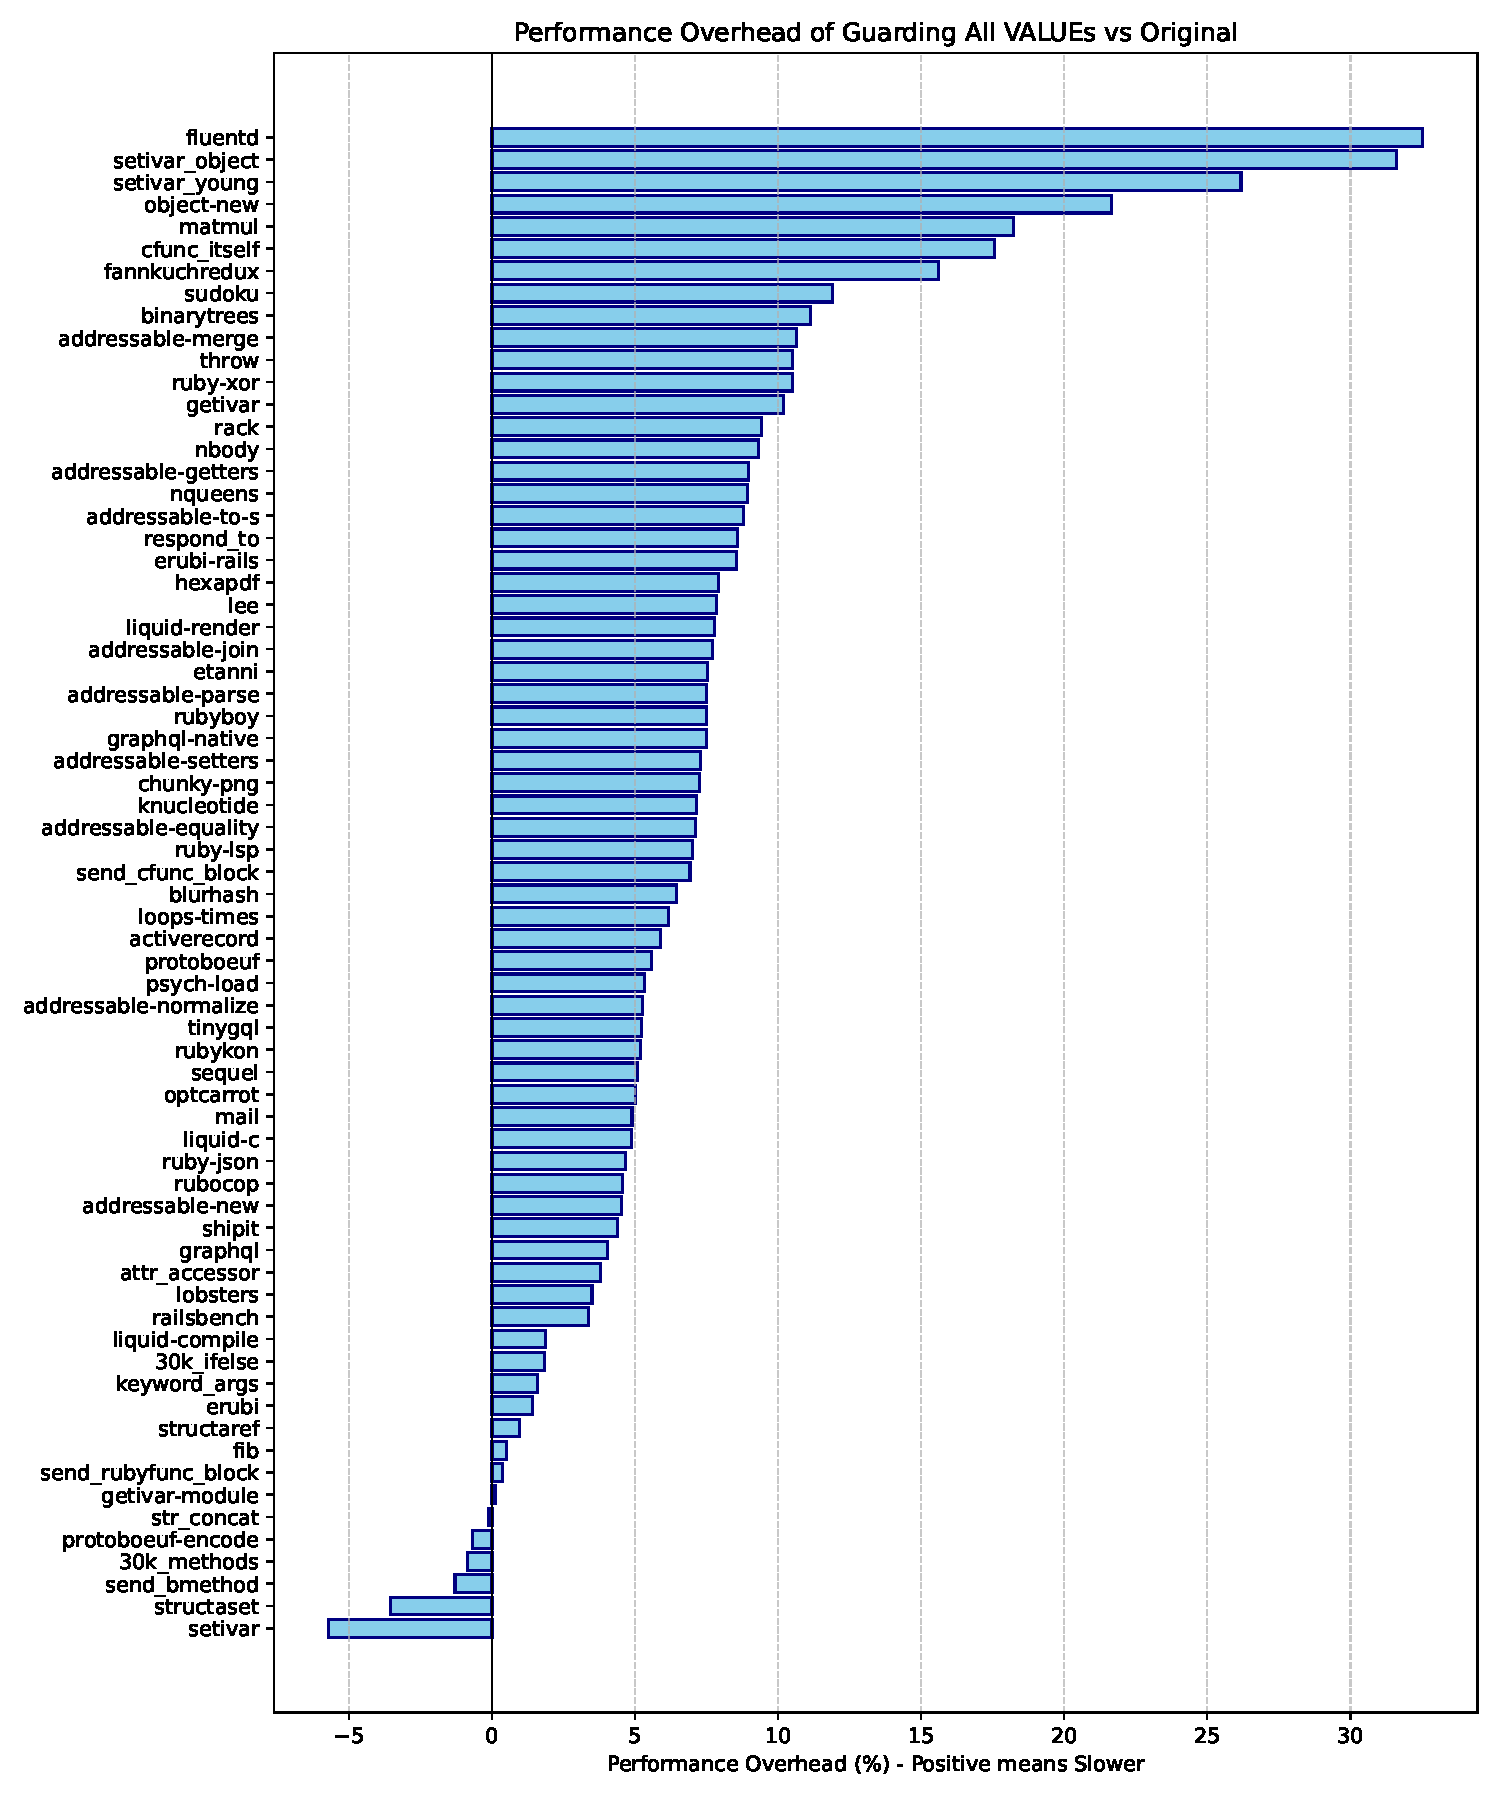
\includegraphics[width=\linewidth]{benchmark_comparison.pdf}
\caption{Performance change from guarding all VALUEs relative to the original CRuby (positive values indicate slowdown).}
\label{fig:benchmark_comparison}
\end{figure}

The slowdown is benchmark-dependent because the additional spill/reload and inhibited optimizations matter most when the baseline work per iteration is small and the affected VM primitive sits on the hot path. In ruby-bench, \texttt{setivar\_young} and \texttt{setivar\_object} are microbenchmarks intended to stress instance-variable writes and the GC write-barrier path by setting an instance variable to a heap object (rather than an immediate), which requires write-barrier bookkeeping.\footnote{\url{https://github.com/ruby/ruby-bench/blob/main/benchmarks.yml} and benchmark sources.} Because these benchmarks measure a tight loop whose body is essentially ``set ivar + barrier,'' any additional per-iteration overhead introduced in the corresponding C fast path (including extra stack traffic from pervasive guards) appears almost directly as a large percentage slowdown.

The \texttt{fluentd} benchmark, in contrast, is a macrobenchmark derived from a production log collector workload that parses logs and forwards them to destinations. Such pipelines are CPU-intensive, and this style of workload allocates and manipulates large numbers of strings and hashes, spending much of its time in C implementations of core operations and exercising GC frequently.  Consequently, a global ``guard-everything'' modification affects many hot runtime functions (not just a single site), and the aggregate cost compounds across the workload.

These results suggest that indiscriminate guarding can harm the interpreter's performance. This motivates a tool that helps focus review on likely omission sites and highlights candidates for cleanup.
